\chapter{Leçon 21: Am Restaurant an an der Gemeng}

\section{Am Restaurant / Au Restaurant / At the Restaurant}

Eng Famill geet an de Restaurant. \textit{Une famille va au restaurant. / A family goes to the restaurant.}

\begin{itemize}
    \item \textbf{Garçon:} Gudden Owend! Wëllkomm. En Dësch fir véier? \textit{(Bonsoir ! Bienvenue. Une table pour quatre ? / Good evening! Welcome. A table for four?)}
    \item \textbf{Fra:} Jo, e groussen Dësch. An hutt Dir e Babystull fir dee Klengen? \textit{(Oui, une grande table. Et avez-vous une chaise pour bébé pour le petit ? / Yes, a large table. And do you have a baby chair for the little one?)}
    \item \textbf{Garçon:} Natierlech, Madame. Wat wëllt Dir drénken? \textit{(Naturellement, Madame. Que voulez-vous boire ? / Naturally, Madam. What would you like to drink?)}
    \item \textbf{Fra:} Plat Waasser fir jiddereen. Mir liewe gesond. \textit{(De l'eau plate pour tout le monde. Nous vivons sainement. / Still water for everyone. We live healthily.)}
    \item \textbf{Garçon:} Wëllt Dir eise gudde Wäin probéieren? Eng Fläsch oder e Glas? De Bordeau ass ganz gutt. \textit{(Voulez-vous essayer notre bon vin ? Une bouteille ou un verre ? Le Bordeaux est très bon. / Do you want to try our good wine? A bottle or a glass? The Bordeaux is very good.)}
    \item \textbf{Mann:} Ah, e Glas Rouden, wannechgelift. \textit{(Ah, un verre de rouge, s'il vous plaît. / Ah, a glass of red, please.)}
    \item \textbf{Garçon:} An de Bordeau fir den Här. \textit{(Et le Bordeaux pour le monsieur. / And the Bordeaux for the gentleman.)}
    \item \textbf{Fra:} Nee, nee! Mir fueren Auto, an ech hu kee Führerschäin. Et gëtt kee Wäin fir hien. \textit{(Non, non ! Nous conduisons, et je n'ai pas de permis de conduire. Il n'y aura pas de vin pour lui. / No, no! We are driving, and I have no driver's license. There will be no wine for him.)}
    \item \textbf{Mann:} Ma, op d'mannst e bësse Spruddelwaasser? \textit{(Eh bien, au moins un peu d'eau gazeuse ? / Well, at least some sparkling water?)}
    \item \textbf{Fra:} OK, Spruddelwaasser, awer net ze vill. \textit{(OK, de l'eau gazeuse, mais pas trop. / OK, sparkling water, but not too much.)}
\end{itemize}

\vspace{0.5em}
\textbf{D'Iessen bestellen / Commander le repas / Ordering the meal}
\vspace{0.5em}

\begin{itemize}
    \item \textbf{Garçon:} An ze iessen? Mir hu gutt Roudfleesch. Zum Beispill Bifdeck, Réi, an Hammelfleesch. \textit{(Et à manger ? Nous avons de la bonne viande rouge. Par exemple du bifteck, du chevreuil, et du mouton. / And to eat? We have good red meat. For example steak, venison, and mutton.)}
    \item \textbf{Mann:} Oh, ech huelen eng Bouchée à la reine! \textit{(Oh, je prends une bouchée à la reine ! / Oh, I'll take a bouchée à la reine!)}
    \item \textbf{Fra:} Dat ass ze vill Fett. Du hëls eng Zaloot mat Gromperen! \textit{(C'est trop de gras. Tu prends une salade avec des pommes de terre ! / That's too much fat. You're taking a salad with potatoes!)}
    \item \textbf{Mann:} ...OK, eng Zaloot. \textit{(...OK, une salade. / ...OK, a salad.)}
    \item \textbf{Teenager:} Ech wëll Gegrilltfleesch mat Fritten! Schwéngsfleesch! \textit{(Je veux de la viande grillée avec des frites ! De la viande de porc ! / I want grilled meat with fries! Pork!)}
    \item \textbf{Garçon:} Et deet mer Leed, Gegrilltfleesch ass am Moment aus. \textit{(Je suis désolé, la viande grillée est épuisée en ce moment. / I am sorry, grilled meat is out of stock at the moment.)}
    \item \textbf{Teenager:} Dann huelen ech e Bifdeck. \textit{(Alors je prends un bifteck. / Then I'll take a steak.)}
    \item \textbf{Garçon:} Wéi gebroden? \textit{(Quelle cuisson ? / How cooked?)}
    \item \textbf{Teenager:} Medium. \textit{(À point. / Medium.)}
    \item \textbf{Garçon:} An fir dat Klengt? \textit{(Et pour le petit ? / And for the little one?)}
    \item \textbf{Fra:} Fir de Klengen: Spaghetti. \textit{(Pour le petit : spaghetti. / For the little one: spaghetti.)}
    \item \textbf{Kand:} Ech wëll Mëllech! \textit{(Je veux du lait ! / I want milk!)}
    \item \textbf{Fra:} Nëmmen ouni Laktos. Hutt Dir Sojamëllech? \textit{(Seulement sans lactose. Avez-vous du lait de soja ? / Only lactose-free. Do you have soy milk?)}
    \item \textbf{Garçon:} Jo, Madame. \textit{(Oui, Madame. / Yes, Madam.)}
\end{itemize}

\vspace{0.5em}
\textbf{Nom Iessen / Après le repas / After the meal}
\vspace{0.5em}

\begin{itemize}
    \item \textbf{Garçon:} Wëllt Dir nach en Dessert? \textit{(Voulez-vous encore un dessert ? / Would you like a dessert?)}
    \item \textbf{Mann:} Ech hätt gär en Tiramisu! \textit{(J'aimerais bien un tiramisu ! / I would like a tiramisu!)}
    \item \textbf{Fra:} Kee Kaffi a keen Zocker fir hien, soss kënne mir net schlofen. Nëmmen Uebst. \textit{(Pas de café et pas de sucre pour lui, sinon nous ne pourrons pas dormir. Seulement des fruits. / No coffee and no sugar for him, otherwise we won't be able to sleep. Only fruit.)}
    \item \textbf{Garçon:} E klenge Digestif fir den Här? \textit{(Un petit digestif pour le monsieur ? / A small digestif for the gentleman?)}
    \item \textbf{Fra:} Hien huet gesot nee! \textit{(Il a dit non ! / He said no!)}
    \item \textbf{Garçon:} Gutt, gutt... d'Rechnung? \textit{(Bien, bien... l'addition ? / Good, good... the bill?)}
    \item \textbf{Mann:} Jo, wannechgelift. \textit{(Oui, s'il vous plaît. / Yes, please.)}
    \item \textbf{Garçon:} Dat mécht 141 Euro. \textit{(Cela fait 141 euros. / That is 141 euros.)}
    \item \textbf{Mann:} Da soen ech villmools Merci. An entschëllegt fir... alles. \textit{(Alors je vous remercie beaucoup. Et désolé pour... tout. / Then thank you very much. And sorry for... everything.)}
\end{itemize}

\vspace{1cm}

\section{An der Gemeng / À la Commune / At the Population Office}

E Mann geet op d'Gemeng fir seng Famill unzemellen. Et gëtt awer eng Iwwerraschung... \textit{Un homme va à la commune pour inscrire sa famille. Mais il y a une surprise... / A man goes to the municipality to register his family. But there is a surprise...}

\begin{itemize}
    \item \textbf{Beamten:} Moien. Woumat kann ech Iech hëllefen? \textit{(Bonjour. En quoi puis-je vous aider ? / Hello. How can I help you?)}
    \item \textbf{Mann:} Moien, ech wëll meng Fra, meng véier Kanner, a mech hei an der Gemeng umellen. \textit{(Bonjour, je veux m'inscrire moi, ma femme et mes quatre enfants ici dans la commune. / Hello, I want to register my wife, my four children, and myself here in the municipality.)}
    \item \textbf{Beamten:} Gutt. Hutt Dir Äre Pass an d'Päss vun Ärer Famill dobäi? \textit{(Bien. Avez-vous votre passeport et les passeports de votre famille avec vous ? / Good. Do you have your passport and the passports of your family with you?)}
    \item \textbf{Mann:} Jo, hei sinn d'Päss. \textit{(Oui, voici les passeports. / Yes, here are the passports.)}
    \item \textbf{Beamten:} Huet Är Fra e gëltege Visa? Wou hutt Dir virdru gewunnt? \textit{(Votre femme a-t-elle un visa valide ? Où avez-vous vécu avant ? / Does your wife have a valid visa? Where did you live before?)}
    \item \textbf{Mann:} Jo, si huet e gëltege Visa. Mir hunn am Ausland gewunnt. \textit{(Oui, elle a un visa valide. Nous vivions à l'étranger. / Yes, she has a valid visa. We lived abroad.)}
    \item \textbf{Beamten:} Wéi ass Är nei Adress? Dir braucht eng grouss Wunneng fir véier Kanner. \textit{(Quelle est votre nouvelle adresse ? Vous avez besoin d'un grand appartement pour quatre enfants. / What is your new address? You need a large apartment for four children.)}
    \item \textbf{Mann:} An der Haaptstrooss 10. Et ass grouss genuch. \textit{(Dans la rue principale 10. C'est assez grand. / In the main street 10. It is big enough.)}
    \item \textbf{Beamten:} Da musst Dir dëse Formulaire ausfëllen. A ween ass nach op dëser Lëscht hei? Do steet de Numm "Fluffy". Ass dat Äert fënneft Kand? \textit{(Alors vous devez remplir ce formulaire. Et qui d'autre est sur cette liste ici ? Il y a le nom "Fluffy". Est-ce votre cinquième enfant ? / Then you must fill out this form. And who else is on this list here? There is the name "Fluffy". Is that your fifth child?)}
    \item \textbf{Mann:} Ah, nee. De Fluffy ass eise Python. Eise Hausdéier. \textit{(Ah, non. Fluffy est notre python. Notre animal de compagnie. / Ah, no. Fluffy is our python. Our pet.)}
    \item \textbf{Beamten:} E Python?! Eng Schlaang? \textit{(Un python ?! Un serpent ? / A python?! A snake?)}
    \item \textbf{Mann:} Jo. Muss ech hien och umellen? Hien ass frëndlech... \textit{(Oui. Dois-je l'inscrire aussi ? Il est amical... / Yes. Do I have to register him too? He is friendly...)}
    \item \textbf{Beamten:} Et deet mer Leed, mir hu keng Kategorien fir Schlaangen. Stellt Iech vir, jidderee bréngt e Python mat an d'Schlaang fir ze waarden! \textit{(Je suis désolé, nous n'avons pas de catégories pour les serpents. Imaginez si tout le monde amenait un python dans la file d'attente ! / I am sorry, we don't have categories for snakes. Imagine if everyone brought a python into the waiting queue!)}
    \item \textbf{Mann:} A wou ass de Problem? De Fluffy ass hei a menger Täsch. \textit{(Et où est le problème ? Fluffy est ici dans mon sac. / And where is the problem? Fluffy is here in my bag.)}
    \item \textbf{Beamten:} Waat?! Wannechgelift, maacht d'Täsch zou. Fëllt just de Formulaire fir d'Mënschen aus! \textit{(Quoi ?! S'il vous plaît, fermez le sac. Remplissez juste le formulaire pour les humains ! / What?! Please, close the bag. Just fill out the form for the humans!)}
\end{itemize}

\vspace{1cm}

\section{Verschidde Wierder an Ausdréck / Mots et Expressions Diverses / Various Words and Expressions}

\begin{itemize}
    \item \textbf{Ech schaffen am Gaart.} $\rightarrow$ Je travaille dans le jardin. / I am working in the garden.
    \item \textbf{Zéien / Drécken} $\rightarrow$ Tirer / Pousser. / To pull / To push.
    \item \textbf{Zielen} $\rightarrow$ Compter, Raconter. / To count, to tell (a story).
    \item \textbf{D'Zuelen} $\rightarrow$ Les nombres, les chiffres. / The numbers.
    \item \textbf{Zéng} $\rightarrow$ Dix. / Ten. \textit{(Bemierkung: net 'zeng' / Note: not 'zeng')}
    \item \textbf{Beschtellen / Buchen / Reservéieren} $\rightarrow$ Commander / Réserver (un vol) / Réserver (une table). / To order / To book / To reserve.
    \item \textbf{Empfeelen} $\rightarrow$ Recommander. / To recommend.
\end{itemize}

\vspace{1.5cm}
\color{geminiBlue}\hrule height 1.5pt \vspace{0.5em}\color{black}
\section{Vokabulär: Neit Wierderbuch}

\begin{itemize}
    \item \textbf{e Pass} (Pl.: d'Päss) $\rightarrow$ un passeport (a passport)
    \item \textbf{den Zocker} $\rightarrow$ le sucre (the sugar)
    \item \textbf{eng Schlaang} (Pl.: d'Schlaangen) $\rightarrow$ une file d'attente (a queue) ODER un serpent (a snake)
\end{itemize}

\vspace{1em}

\begin{center}
    \begin{minipage}[t]{0.48\textwidth}
        \centering
        \framebox{\parbox{0.9\linewidth}{\centering
            \vspace{0.5cm}
            % Note: Please ensure the generated image 'pass.png' is in the vokab_300dpi directory.
            
\includegraphics[width=0.9\linewidth]{vokab_300dpi/pass.png} \\
            \small\textit{E Pass (Un passeport / A passport)}
            \vspace{0.5cm}
        }}
    \end{minipage}
    \hfill
    \begin{minipage}[t]{0.48\textwidth}
        \centering
        \framebox{\parbox{0.9\linewidth}{\centering
            \vspace{0.5cm}
            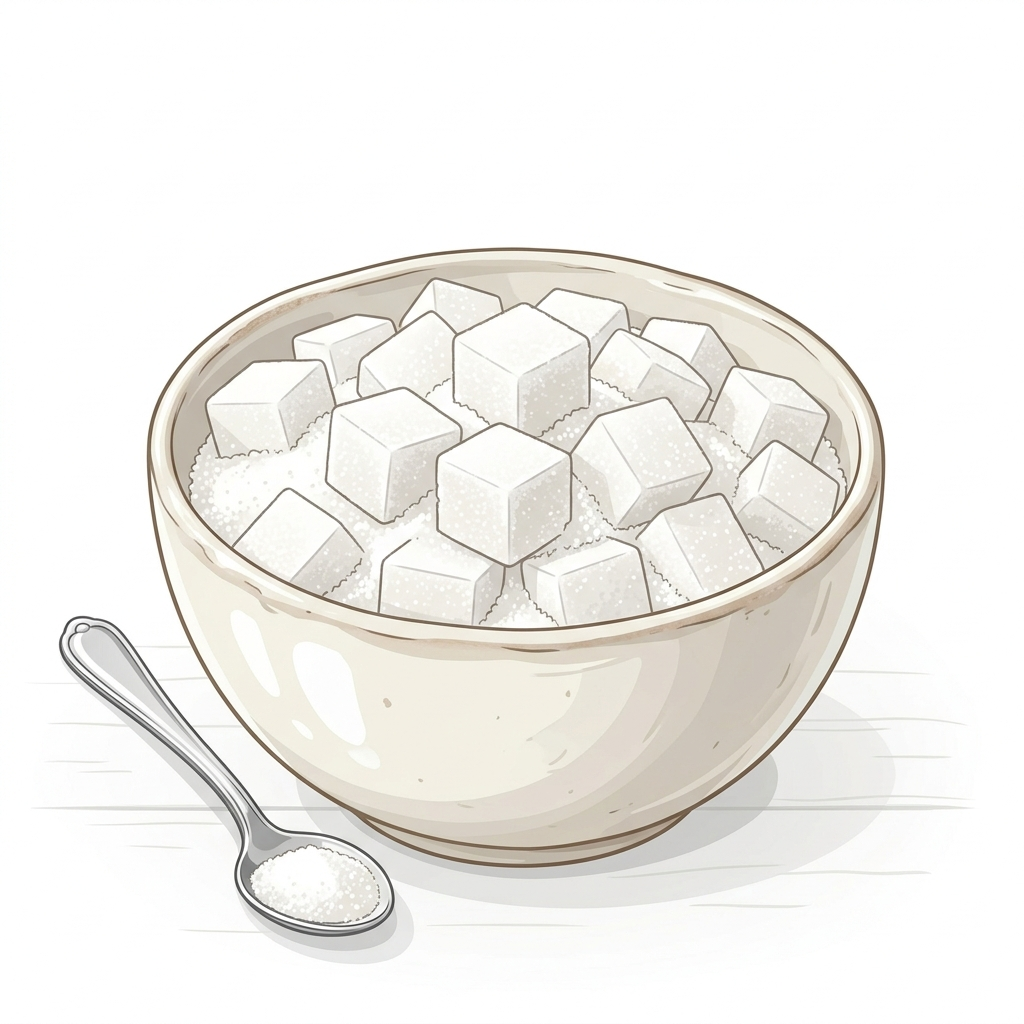
\includegraphics[width=0.9\linewidth]{vokab_300dpi/zocker.png} \\
            \small\textit{Den Zocker (Le sucre / The sugar)}
            \vspace{0.5cm}
        }}
    \end{minipage}
    
    \vspace{1em}
    
    \begin{minipage}[t]{0.48\textwidth}
        \centering
        \framebox{\parbox{0.9\linewidth}{\centering
            \vspace{0.5cm}
            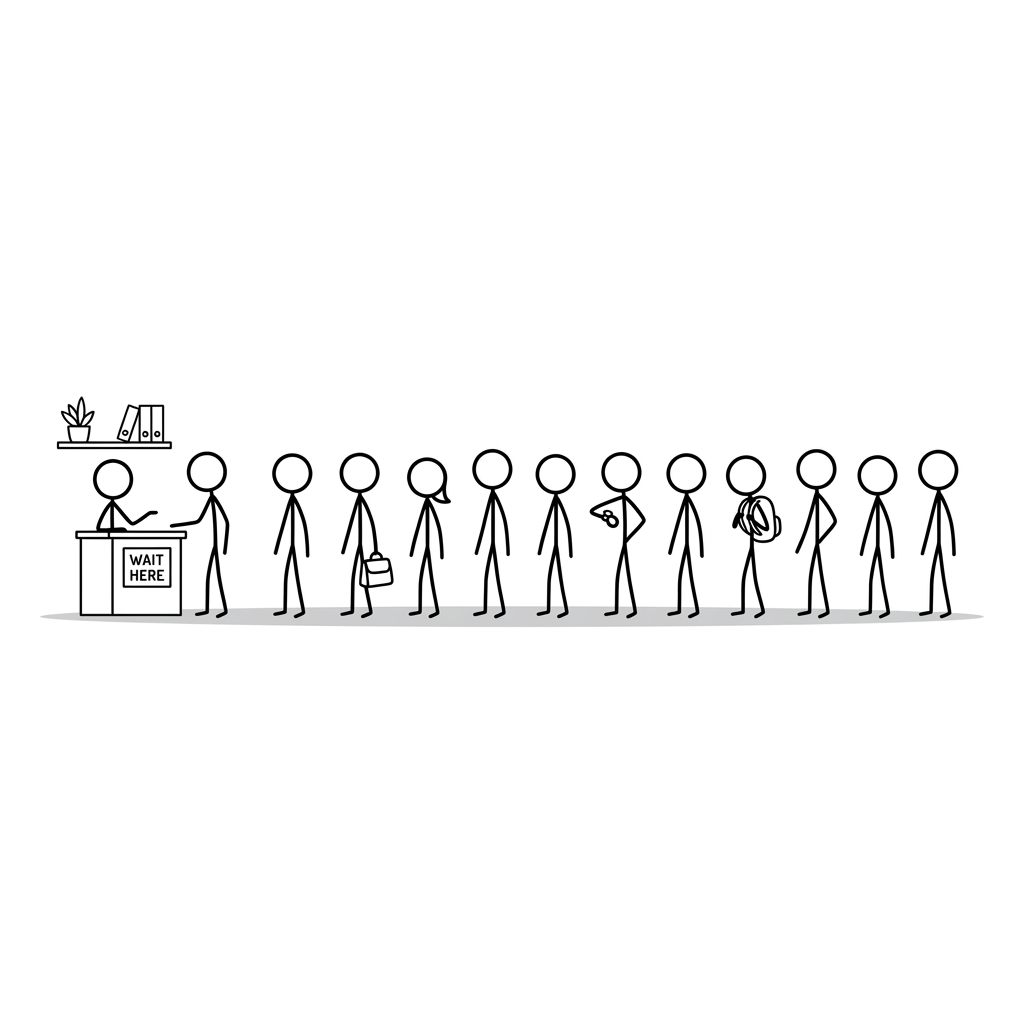
\includegraphics[width=0.9\linewidth]{vokab_300dpi/schlaang_queue.png} \\
            \small\textit{Eng Schlaang (Une file d'attente / A queue)}
            \vspace{0.5cm}
        }}
    \end{minipage}
    \hfill
    \begin{minipage}[t]{0.48\textwidth}
        \centering
        \framebox{\parbox{0.9\linewidth}{\centering
            \vspace{0.5cm}
            
\includegraphics[width=0.9\linewidth]{vokab_300dpi/schlaang_snake.png} \\
            \small\textit{Eng Schlaang (Un serpent / A snake)}
            \vspace{0.5cm}
        }}
    \end{minipage}
\end{center}
